\documentclass[cours, noCustomPackages]{UPSTI_Document}
\usepackage{IUT_Annecy}
\usepackage{logos_iut}

% --- Git info (nécessite git et les hooks gitinfo2 activés) ---
\usepackage{gitinfo2} % génère gitHeadInfo.gin via hooks post-commit/checkout/merge
% Voir doc gitinfo2 pour activer les hooks une fois:
%   git config --local gitinfo2.enabled true
%   git info # ou copier les hooks fournis par le package
\newcommand{\UPSTItitreEnTete}{Chaîne de conversion -- Cellule robotique}
\newcommand{\UPSTItitre}{De la donnée NOC au bloc fonctionnel : comprendre la chaîne de conversion}
\newcommand{\UPSTItitreEnTetePages}{Chaîne de conversion NOC -- Code applicatif}
\newcommand{\UPSTIsousTitreEnTete}{Préparation -- HMI et robot}

% Trou de complétion inséré DANS un listing, au point exact où l'étudiant
% doit écrire (même principe que dans le DS1 S1) : escapeinside dédié à ce
% document, avec un délimiteur `(*@...@*)` qui ne peut pas être confondu
% avec un commentaire ST normal `(* ... *)`.
\lstset{escapeinside={(*@}{@*)}}
% Syntaxe : \trou[reponse]{largeur}
%   - version élève (\documentVersion{E}) : rectangle vide (réponse ignorée) ;
%   - version prof  (\documentVersion{P}) : réponse affichée en rouge dans
%     le rectangle (via \UPSTIcorrection), qui s'élargit si nécessaire.
% Dans un listing, la réponse est en mode LaTeX : échapper les « _ » (\_).
\newcommand{\trou}[2][]{%
    \tikz[baseline=(trou.base)]{%
        \node[draw=gray!70, dashed, rounded corners=2pt, inner sep=2pt,
              minimum width=#2, minimum height=1.6em, fill=white,
              anchor=base] (trou) {\strut\ifnumequal{1}{\UPSTIidVersionDocumentDef}%
                {\UPSTIcorrection[1]{\ttfamily #1}}{}};%
    }%
}

\discipline[Autom - Robotique]{Automatisme pour la robotique}
\graphicspath{{images/}}

% \providecommand : ne définit une valeur par défaut que si le préambule local
% (input{preamble.tex}) n'a pas déjà défini \UPSTItitreEnTete, afin que ce
% fichier de préambule de module reste réutilisable par tous les sous-dossiers.
\providecommand{\UPSTItitreEnTete}{EthernetIP}


\newcommand{\basepath}{U:\textbackslashDocuments\textbackslashBUT\textbackslashGEII\textbackslashModulesS5\textbackslashAutomatisme_Pour_Robotique\textbackslash}
\newcommand{\subdir}[1]{\basepath{}#1}


%%% Définition du langage ST %%%
%New colors defined below
\definecolor{codegreen}{rgb}{0,0.6,0}
\definecolor{codegray}{rgb}{0.5,0.5,0.5}
\definecolor{codepurple}{rgb}{0.502,0.502,0.0}
\definecolor{backcolour}{rgb}{0.95,0.95,0.95}

\lstdefinelanguage{ST}
{
	morekeywords={
	case,of,if,then,end_if,end_case,super,function_block,extends,var,
	constant, byte,,end_var,var_input, real,bool,var_output,
	dint,udint,word,dword,array, of,uint,not,adr, program, for, end_for, while, do, end_while, repeat, end_repeat, until, to, by, else, elsif, var_in_out,interface,method,property
	},
	otherkeywords={
		:, :=, <>,;,\,.,\[,\],\^,1,2,3,4,5,6,7,8,9,0,TRUE, FALSE, \{attribute,  \'hide\'\}
	},
	keywords=[1]{
		case,of,if,then,end_if,end_case,super,function_block,extends,var,
		constant, byte,,end_var,var_input, real,bool,var_output,
		dint,udint,word,dword,array, of,uint,not,adr, :, :=, <>,;,\,.,\[,\],\^,program, for, end_for, while, do, end_while, repeat, end_repeat, until, to, by, else, elsif, var_in_out,interface,method,property
	},
	keywordstyle=[1]\color{blue},
	keywords=[2]{
		1,2,3,4,5,6,7,8,9,0, TRUE, FALSE
	},
	keywordstyle=[2]\color{codepurple},
	keywords=[3]{
		\{attribute,  \'hide\'\}
	},
	keywordstyle=[3]\color{codegray},
	sensitive=false,
	morecomment=[l]{//}, 
	morecomment=[s]{(*}{*)},
	morestring=[b]{"},
	morestring=[b]{'}
}

\lstset{
	language={ST},
	backgroundcolor=\color{backcolour},
	commentstyle=\color{codegreen}\textit,
	keywordstyle=\color{blue},
	numberstyle=\tiny\color{codegray},
	stringstyle=\color{codepurple},
	basicstyle=\ttfamily\scriptsize,
	breakatwhitespace=false,         
	breaklines=true,                 
	captionpos=b,                    
	keepspaces=true,                 
	numbers=left,                    
	numbersep=5pt,                  
	showspaces=false,                
	showstringspaces=false,
	showtabs=false,                  
	tabsize=2
}
%\lstMakeShortInline[columns=fixed]~

% Version du document : P = version professeur (corrigés affichés en rouge
% dans les trous et encadrés « Correction » après les questions ouvertes) ;
% remplacer par \documentVersion{E} pour obtenir la version élève.
\documentVersion{P}
\newcommand{\UPSTInumeroVersion}{\gitAuthorDate\if \gitDirty*dirty \fi}
\newcommand{\UPSTInumero}{0.1}
\begin{document}

\tableofcontents
\section{Introduction}
\label{secIntroductionChaine}

Le premier TP a permis de mettre en service la communication avec le
contrôleur \textbf{PFC200} (poste guichet) : chaque bit produit ou
consommé par cet équipement correspond directement à un capteur ou un
actionneur, et un simple \textbf{alias mémoire} (chevauchement d'une
variable structurée sur la zone \texttt{\%MW} du coupleur) suffit à lui
donner un nom exploitable dans le programme.

Ce document prépare la suite des TP, où deux autres équipements du réseau
\texttt{NOC\_ETHIP\_ROBOT} doivent être mis en œuvre : le contrôleur
\textbf{M221} (pupitre opérateur et écran de supervision) et la baie
\textbf{CS9} du robot (serveur \texttt{uniVALplc}). Dans les deux cas, un
alias seul ne suffit plus : les octets échangés ne portent pas
directement une information unitaire exploitable, il faut un
\textbf{bloc fonctionnel de conversion} pour leur donner du sens.

\begin{UPSTIinfor}{Pourquoi un alias ne suffit plus}
Pour le PFC200, chaque bit \emph{est} l'information (un capteur, une
commande). Pour le M221 et pour la baie CS9, les octets échangés sont le
résultat d'un \textbf{encodage} propre à la bibliothèque logicielle de
l'équipement (empaquetage de plusieurs informations dans un même octet,
structures imbriquées, types numériques codés sur plusieurs octets...).
Un alias donne seulement accès à cette zone \textbf{brute} : il faut un
bloc fonctionnel qui la décode (en lecture) ou qui l'encode (en écriture)
pour manipuler des informations ayant un nom et un type clairs dans le
programme.
\end{UPSTIinfor}

Ce document traite cette chaîne de conversion dans l'ordre suivant :

\begin{enumerate}
    \item le contrôleur \textbf{M221} (blocs \texttt{FB\_ReadHmi} et
    \texttt{FB\_WriteHmi}), le cas le plus simple des deux ;
    \item la baie \textbf{CS9} (blocs \texttt{VAL\_ReadAxesGroup} et
    \texttt{VAL\_WriteAxesGroup}), plus riche ;
    \item un schéma de synthèse comparant les trois chaînes de conversion
    rencontrées (PFC200, M221, CS9) ;
    \item un TD d'application, sur la mise en œuvre du mode GEMMA
    \textbf{A6} (mise en conditions initiales) du robot.
\end{enumerate}

\section{Rappel : fonctions et blocs fonctionnels}
\label{secRappelBlocsFonctionnels}

Les chaînes de conversion étudiées dans ce document reposent sur des
\textbf{blocs fonctionnels} (\emph{function blocks}, norme IEC~61131-3).
Avant d'aller plus loin, il est utile d'en rappeler la nature exacte et de
la comparer à celle d'une simple fonction.

\begin{UPSTIinfor}{Fonction ou bloc fonctionnel ?}
\begin{description}
    \item[Fonction] Ne possède \textbf{aucune mémoire} entre deux appels :
    son résultat ne dépend que des arguments fournis à l'appel en cours.
    Elle ne peut retourner qu'une seule valeur (éventuellement composée),
    directement, par son nom.
    \item[Bloc fonctionnel] Est \textbf{instancié} (une variable, de type
    bloc fonctionnel, doit être déclarée) et \textbf{conserve un état}
    entre deux appels successifs : fronts montants mémorisés, étapes d'une
    temporisation, dernière erreur rencontrée... Il peut exposer plusieurs
    sorties simultanément (\texttt{VAR\_OUTPUT}) et, pour les blocs étudiés
    ici, des paramètres \texttt{VAR\_IN\_OUT} qu'il lit \emph{et} modifie.
\end{description}
\end{UPSTIinfor}

Tous les blocs rencontrés dans ce document et dans les TP suivants sont
des blocs fonctionnels. C'est en particulier le cas des blocs \texttt{MC\_}
(un bloc de mouvement doit savoir, d'un cycle à l'autre, s'il a déjà
démarré le mouvement demandé, afin de ne déclencher l'exécution que sur un
\textbf{front montant} de son entrée \texttt{Execute}) : une fonction,
sans mémoire, ne pourrait pas détecter ce front.

\begin{UPSTIactivite}[4][Fonction ou bloc fonctionnel ?][][][TD]
\UPSTIquestion{Les éléments suivants sont tous utilisés dans les TP de la
cellule. Pour chacun, indiquer s'il s'agit d'une \textbf{fonction} (appel
direct, résultat récupéré dans une variable) ou d'un \textbf{bloc
fonctionnel} (instance à réserver dans l'éditeur de données, onglet
\emph{Bloc fonction}), en justifiant en une phrase par le critère de
mémorisation d'état :
\begin{enumerate}
    \item \texttt{InitChart}, appelé au premier cycle pour initialiser le
    GEMMA, dont la valeur de retour est récupérée dans un objet
    \texttt{xResult : BOOL} ;
    \item \texttt{MC\_GroupReset}, déclenché sur front montant de son
    entrée \texttt{Execute} ;
    \item \texttt{TON}, temporisateur standard IEC~61131-3, dont la sortie
    \texttt{Q} passe à \texttt{TRUE} lorsque son entrée \texttt{IN} est restée
    à \texttt{TRUE} pendant au moins la durée \texttt{PT} ;
    \item la détection du front montant du bouton « Arrêt demandé » du
    pupitre.
\end{enumerate}}
\UPSTIquadrillage{4}

\begin{UPSTIcorrectionP}{Corrigé}
\begin{enumerate}
    \item \texttt{InitChart} est une \textbf{fonction} : elle est appelée
    directement (pas d'instance) et retourne une unique valeur
    \texttt{BOOL} récupérée dans \texttt{xResult} ; son action (rendre
    actif l'état initial du graphe passé en argument) ne nécessite aucune
    mémoire d'un appel à l'autre.
    \item \texttt{MC\_GroupReset} est un \textbf{bloc fonctionnel} : pour
    ne réagir qu'au \textbf{front montant} d'\texttt{Execute}, il doit
    mémoriser la valeur d'\texttt{Execute} au cycle précédent (et l'état
    d'avancement de sa requête) -- d'où l'instance
    \texttt{InstGroupResetD2} à réserver.
    \item \texttt{TON} est un \textbf{bloc fonctionnel} : pour savoir si
    \texttt{IN} est à \texttt{TRUE} depuis au moins \texttt{PT}, il doit
    mémoriser d'un cycle à l'autre le temps écoulé depuis lequel
    \texttt{IN} est à \texttt{TRUE} -- une fonction, qui ne voit que la
    valeur courante de \texttt{IN}, en serait incapable.
    \item La détection de front montant est un \textbf{bloc fonctionnel}
    (\texttt{R\_TRIG}) : détecter un front, c'est comparer la valeur
    courante à celle du cycle précédent, qui doit donc être mémorisée.
\end{enumerate}
\end{UPSTIcorrectionP}

\UPSTIquestion{Le mode D2 du TP~3 utilise les blocs
\texttt{MC\_GroupReset}, \texttt{MC\_GroupStop} et
\texttt{MC\_GroupContinue}. En respectant la règle de nommage imposée
(nom d'instance faisant référence au mode, par exemple
\texttt{InstGroupResetD2}), écrire la déclaration des trois instances
nécessaires.}

\begin{lstlisting}
VAR
    (*@\trou[InstGroupResetD2]{4cm}@*) : (*@\trou[MC\_GroupReset]{3.5cm}@*);
    (*@\trou[InstGroupStopD2]{4cm}@*) : (*@\trou[MC\_GroupStop]{3.5cm}@*);
    (*@\trou[InstGroupContinueD2]{4cm}@*) : (*@\trou[MC\_GroupContinue]{3.5cm}@*);
END_VAR
\end{lstlisting}
\end{UPSTIactivite}

\UPSTIremarque[Préfixes de bibliothèque]{Les blocs fonctionnels utilisés
sur la cellule suivent une convention de préfixe selon leur origine :
\texttt{VAL\_} pour la bibliothèque \texttt{uniVALplc} du robot,
\texttt{MC\_} pour les blocs \texttt{Motion Control} conformes au standard
PLCopen, \texttt{FB\_} pour les blocs maison de l'application.}

\section{Notations imposées pour les noms}
\label{secNotations}

\begin{UPSTIinfor}{Une notation imposée, à respecter dans vos propres programmes}
Les noms de variables, de types, d'objets et d'instances utilisés dans ce document
(\texttt{stopRequest}, \texttt{resetD2}, \texttt{staeubliRobotScara}...) ne sont
pas choisis au hasard : ils suivent les conventions de nommage imposées dans les TP (document
« Conventions de nommage »). Le type d'une variable n'est \textbf{pas} encodé dans son nom
(l'environnement de développement l'affiche) : un nom décrit son rôle métier, en camelCase.
Vous devez appliquer ces mêmes règles pour nommer vos propres variables et instances dans le TD.
\end{UPSTIinfor}

\subsection{Variables obtenues par IO-Scanning}
\label{secNotationsIoScanning}

\begin{center}
    \begin{tabular}{|p{2.8cm}|p{6.5cm}|p{5cm}|}
        \hline
        \textbf{Préfixe} & \textbf{Signification} & \textbf{Exemple} \\
        \hline
        \texttt{in<Nom>} & Entrée booléenne autonome produite par un équipement scruté. & \texttt{inAid}, \texttt{inDgt} \\
        \hline
        \texttt{out<Nom>} & Sortie booléenne autonome consommée par un équipement scruté. & \texttt{outBE}, \texttt{outBP} \\
        \hline
        \texttt{<nom>} & Entrée / sortie du pupitre HMI, en tant que champ des structures dédiées \texttt{inputs} / \texttt{outputs} : pas de préfixe. & \texttt{j1Plus}, \texttt{auto}, \texttt{redColumn} \\
        \hline
    \end{tabular}
\end{center}

\subsection{Types et champs de structure}
\label{secNotationsTypes}

\begin{center}
    \begin{tabular}{|p{2.8cm}|p{6.5cm}|p{5cm}|}
        \hline
        \textbf{Préfixe de type} & \textbf{Signification} & \textbf{Exemple} \\
        \hline
        \texttt{T<Nom>} & Type maison, défini par le développeur de l'application (STRUCT ou enum). & \texttt{THmi}, \texttt{THmiInputs}, \texttt{TCtrlStatusGroup}, \texttt{TMoveAbsolute} \\
        \hline
        \texttt{T\_<Nom>} & Type de la bibliothèque \texttt{uniVALplc} (Stäubli). & \texttt{T\_StaeubliRobot}, \texttt{T\_FromRobot}, \texttt{T\_ToRobot}, \texttt{T\_CartesianPos}, \texttt{T\_JointPos}, \texttt{T\_Trsf} \\
        \hline
    \end{tabular}
\end{center}

Les champs d'une structure portent simplement leur \textbf{nom métier} en camelCase, avec une
minuscule initiale, sans préfixe ni lettre de type :

\begin{center}
    \begin{tabular}{|p{2.8cm}|p{3.2cm}|p{8.3cm}|}
        \hline
        \textbf{Type du champ} & \textbf{Forme} & \textbf{Exemple} \\
        \hline
        \texttt{BOOL} & \texttt{<nom>} & \texttt{enable}, \texttt{busy}, \texttt{done}, \texttt{error}, \texttt{execute} \\
        \hline
        \texttt{INT} & \texttt{<nom>} & \texttt{stateGmma}, \texttt{partNumber} \\
        \hline
        \texttt{UINT} / \texttt{UDINT} & \texttt{<nom>} & \texttt{coordSystem}, \texttt{bufferMode}, \texttt{errorID} \\
        \hline
        \texttt{REAL} / \texttt{TIME} & \texttt{<nom>} & \texttt{velocity}, \texttt{acceleration}, \texttt{elapsedTime} \\
        \hline
        \texttt{ARRAY} & \texttt{<nom>} & \texttt{hex7Seg} \\
        \hline
        Type composé & \texttt{<nom>} & \texttt{cartesianPos} (\texttt{T\_CartesianPos}), \texttt{inputs} (\texttt{THmiInputs}) \\
        \hline
    \end{tabular}
\end{center}

\subsection{Objets métier}
\label{secNotationsObjets}

Un objet métier se nomme \texttt{<rôle><Équipement>} en camelCase : \texttt{<rôle>} précise la
nature de l'objet ou le sens de l'échange (\texttt{from} : données produites par l'équipement,
\texttt{to} : données qui lui sont destinées), \texttt{<Équipement>} identifie la station
(\texttt{Scara}).

\begin{center}
    \begin{tabular}{|p{4.6cm}|p{5.4cm}|p{4.2cm}|}
        \hline
        \textbf{Objet} & \textbf{Rôle} & \textbf{Type} \\
        \hline
        \texttt{staeubliRobotScara} & Le robot et son contrôleur CS9. & \texttt{T\_StaeubliRobot} \\
        \hline
        \texttt{fromRobotScara} / \texttt{toRobotScara} & Données lues depuis / écrites vers le robot. & \texttt{T\_FromRobot} / \texttt{T\_ToRobot} \\
        \hline
        \texttt{hmiScara} & État complet du pupitre HMI de la station. & \texttt{THmi} \\
        \hline
    \end{tabular}
\end{center}

\subsection{Instances de blocs fonctionnels}
\label{secNotationsInstances}

Les blocs eux-mêmes sont préfixés selon leur origine : \texttt{VAL\_} (bibliothèque
\texttt{uniVALplc}), \texttt{MC\_} (standard PLCopen \emph{Motion Control}), \texttt{FB\_} (bloc
maison). Le nom d'une \textbf{instance} ne reprend pas le nom technique du bloc : il indique son
\textbf{rôle} (fonction résumée en un mot) suivi du mode GEMMA qui l'utilise. L'objet
\texttt{TCtrlStatusGroup} qui regroupe ses paramètres est préfixé par \texttt{status}.

\begin{center}
    \begin{tabular}{|p{4.4cm}|p{6cm}|p{3.8cm}|}
        \hline
        \textbf{Convention} & \textbf{Signification} & \textbf{Exemple} \\
        \hline
        \texttt{<rôle><Mode>} & Instance d'un bloc fonctionnel, suffixée par le mode qui l'utilise. & \texttt{resetD2} (\texttt{MC\_GroupReset}, mode D2) \\
        \hline
        \texttt{status<Rôle><Mode>} & Objet \texttt{TCtrlStatusGroup} de passage de paramètres, suffixé par le rôle et le mode. & \texttt{statusResetD2}, \texttt{statusStopF4} \\
        \hline
    \end{tabular}
\end{center}

\UPSTIremarque[Instances communes à tous les modes]{%
Une instance qui n'est pas propre à un mode (lecture/écriture Ethernet/IP en début et fin de
cycle, mise sous puissance) n'a pas de suffixe de mode : \texttt{readAxes},
\texttt{writeAxes}, \texttt{power} et son objet \texttt{statusPower},
comme \texttt{statusRead}/\texttt{statusWrite} dans le document « Conventions de
nommage ».}

\subsection{Sections et transitions du GEMMA}
\label{secNotationsGmma}

Dans la section SFC \texttt{GM\_Gmma}, l'étape associée au mode \texttt{<Mode>} se nomme
\texttt{GM\_S\_<Mode>} (ex. \texttt{GM\_S\_D2}) et la transition entre deux modes
\texttt{GM\_T\_<ModeA>to<ModeB>} (ex. \texttt{GM\_T\_D1toD2}, \texttt{GM\_T\_D2toA5}).

\section{Alias et chevauchement mémoire}
\label{secAliasChevauchement}

Avant de pouvoir convertir quoi que ce soit, il faut d'abord pouvoir
\textbf{nommer} la zone mémoire brute échangée avec le réseau. C'est le
rôle de l'\textbf{alias}.

\begin{UPSTIinfor}{Alias et chevauchement mémoire}
Sous Control Expert, une variable peut être déclarée par
\textbf{chevauchement} (\emph{overlap}) d'une autre : elle occupe alors
exactement le même espace mémoire que la variable qu'elle chevauche, sans
qu'aucune copie ne soit effectuée. On parle d'\textbf{alias} parce que les
deux variables désignent le même contenu physique sous deux noms et,
éventuellement, deux types différents.

Cette technique est indispensable chaque fois qu'un coupleur réseau
(comme le \texttt{BMX~NOC~0401.2}) ne connaît que des zones \texttt{\%MW}
génériques, numérotées, alors que le programme applicatif a besoin de
noms et de types porteurs de sens.
\end{UPSTIinfor}

\textbf{Exemple.} Le coupleur \texttt{NOC\_ETHIP\_CONVOYEUR} reçoit du
PFC200 un octet de données à l'adresse \texttt{\%MW10} (poids faible). Si
le quatrième bit de cet octet correspond au capteur « palette présente »,
on déclare une variable \texttt{m\_nixPalettePresente} de type
\texttt{BOOL}, chevauchant précisément le bit~3 de \texttt{\%MW10} :

\begin{lstlisting}
m_nixPalettePresente AT %MW10.3 : BOOL;
\end{lstlisting}

Aucune conversion n'est nécessaire ici : le bit \emph{est} directement
l'information recherchée, l'alias suffit à lui donner un nom exploitable
(c'est le cas « à un seul niveau » du PFC200, déjà rencontré en TP1).
C'est précisément lorsque cela ne suffit plus -- lorsque l'information
recherchée est encodée sur plusieurs bits, répartie, ou calculée à partir
d'octets bruts -- qu'un bloc fonctionnel de conversion devient nécessaire,
comme on le verra dans les sections suivantes pour le M221 et pour la baie
CS9.

\begin{UPSTIactivite}[4][Chevauchement sur Schneider M340][][][TD]
\UPSTIquestion{Le coupleur \texttt{NOC\_ETHIP\_CONVOYEUR} reçoit du
PFC200, à l'adresse \texttt{\%MW11}, un octet dont le bit~0 indique l'état
du bouton d'arrêt d'urgence du poste guichet (\texttt{TRUE} = défaut). En
complétant la déclaration ci-dessous, créer un alias
\texttt{m\_nixArretUrgenceGuichet} chevauchant ce bit.}

\begin{lstlisting}
m_nixArretUrgenceGuichet AT (*@\trou{2.2cm}@*) : (*@\trou{1.4cm}@*);
\end{lstlisting}

\UPSTIquestion{Le même octet comporte, sur ses bits~1 et~2, un code sur
2~bits indiquant la couleur de la palette détectée (\texttt{00} = absente,
\texttt{01} = rouge, \texttt{10} = verte, \texttt{11} = bleue). Expliquer
en une phrase pourquoi un simple alias sur ces deux bits ne permettrait
\textbf{pas}, à lui seul, d'obtenir directement une variable
\texttt{m\_couleurPalette} de type énuméré portant les noms
\texttt{ROUGE}/\texttt{VERTE}/\texttt{BLEUE}/\texttt{ABSENTE} : quelle
étape supplémentaire serait alors nécessaire ?}
\end{UPSTIactivite}

\section{Ordre des octets : \emph{big endian} et \emph{little endian}}
\label{secEndianness}

Dès qu'une information occupe \textbf{plusieurs octets} (un entier
16~ou~32~bits, une position cartésienne codée en réel), la conversion ne
se limite plus au découpage bit à bit vu dans la section précédente : il
faut aussi savoir dans quel \textbf{ordre} ranger ces octets en mémoire.

\begin{UPSTIinfor}{\emph{Big endian} / \emph{little endian}}
Pour une donnée multi-octets, deux conventions existent :
\begin{itemize}
    \item \textbf{Big endian} : l'octet de poids \textbf{fort} est stocké
    en premier (à l'adresse la plus basse).
    \item \textbf{Little endian} : l'octet de poids \textbf{faible} est
    stocké en premier.
\end{itemize}
Deux équipements qui échangent une donnée multi-octets doivent
s'accorder sur cette convention, sous peine de lire une valeur
totalement erronée bien que chaque octet, pris isolément, ait été reçu
correctement.
\end{UPSTIinfor}

\textbf{Exemple.} La valeur entière \texttt{0x1234} (4660 en décimal),
codée sur 2~octets, est rangée ainsi :

\begin{center}
\begin{tabular}{|l|c|c|}
\hline
 & \textbf{Octet à l'adresse $n$} & \textbf{Octet à l'adresse $n+1$} \\
\hline
Big endian & \texttt{0x12} & \texttt{0x34} \\
\hline
Little endian & \texttt{0x34} & \texttt{0x12} \\
\hline
\end{tabular}
\end{center}

Un équipement qui interprèterait en \emph{big endian} une donnée envoyée
en \emph{little endian} lirait \texttt{0x3412} (13330) au lieu de
\texttt{0x1234} (4660).

\begin{UPSTIinfor}{Application sur la cellule : configuration du serveur uniVALplc}
Le contrôleur CS9 du robot encode les données échangées via le serveur
\texttt{uniVALplc} selon l'ordre d'octets attendu par le client. Comme
l'automate client de la cellule est un \textbf{M340 de Schneider}
(processeur little endian), l'option \textbf{\emph{Little Endian}} a été
sélectionnée lors de l'installation du serveur \texttt{uniVALplc} sur la
baie CS9 : sans cette configuration, tous les champs numériques
multi-octets de \texttt{T\_StaeubliRobot} (vitesses, positions
cartésiennes, compteurs...) seraient mal interprétés par le programme
Control Expert, même si les blocs \texttt{VAL\_ReadAxesGroup} et
\texttt{VAL\_WriteAxesGroup} sont correctement appelés.
\end{UPSTIinfor}

\begin{UPSTIactivite}[4][Lecture d'une valeur multi-octets][][][TD]
\UPSTIquestion{Le champ \texttt{Status.Heartbeat} de
\texttt{T\_StaeubliRobot} est de type \texttt{UINT}, codé sur 2~octets.
Le coupleur \texttt{NOC\_ETHIP\_ROBOT} reçoit, dans l'ordre, les deux
octets \texttt{0x64} puis \texttt{0x00}. Sachant que le serveur
\texttt{uniVALplc} a été configuré en \emph{little endian}, calculer la
valeur numérique (en décimal) de \texttt{Status.Heartbeat}.}
\UPSTIquadrillage{2.5}

\begin{UPSTIcorrectionP}{Corrigé}
En \emph{little endian}, le premier octet reçu est l'octet de poids
\textbf{faible} : \texttt{0x64} (poids faible) et \texttt{0x00} (poids
fort) donnent \texttt{0x0064}, soit
$6\times16+4 = \mathbf{100}$.
\end{UPSTIcorrectionP}

\UPSTIquestion{Un collègue, en reprenant la configuration du serveur sur
une autre cellule, laisse par erreur l'option \emph{Big Endian}. Quelle
valeur le programme Control Expert lirait-il alors pour
\texttt{Status.Heartbeat}, à partir des mêmes octets \texttt{0x64} puis
\texttt{0x00} ? Ce défaut de configuration serait-il facile à détecter au
premier démarrage de la cellule ? Justifier.}
\UPSTIquadrillage{3.5}

\begin{UPSTIcorrectionP}{Corrigé}
En \emph{big endian}, le premier octet reçu est interprété comme l'octet de
poids \textbf{fort} : le programme lirait \texttt{0x6400}, soit
$100\times256 = \mathbf{25\,600}$.

Ce défaut est \textbf{difficile à détecter} au premier démarrage : chaque
octet est correctement reçu, les bits de santé du coupleur
\texttt{NOC\_ETHIP\_ROBOT} restent à \texttt{TRUE} et les blocs
\texttt{VAL\_ReadAxesGroup}/\texttt{VAL\_WriteAxesGroup} sont appelés
normalement : aucune erreur de communication n'est signalée. Seules des
valeurs numériques \textbf{incohérentes} trahissent le problème (par
exemple une position cartésienne lue sans rapport avec celle affichée sur
le pendant du robot, une vitesse absurde) -- encore faut-il penser à les
comparer. Un champ comme \texttt{Heartbeat}, dont la valeur absolue n'a
pas de signification pour l'opérateur, ne permet pas à lui seul de s'en
apercevoir.
\end{UPSTIcorrectionP}
\end{UPSTIactivite}

\section{Conversion des données du contrôleur M221 (HMI)}
\label{secConversionHmi}

Le contrôleur M221 produit 4 octets et en consomme 40 (cf. document
\texttt{02b\_donnees\_echangees}, section « Données de l'IHM et du
pupitre opérateur »). Ces octets ne sont pas directement exploitables :
ils doivent être lus et écrits à travers les blocs fonctionnels maison
\texttt{FB\_ReadHmi} et \texttt{FB\_WriteHmi}.

\subsection{En lecture}

\begin{enumerate}
    \item L'alias \texttt{fromHmiScara}, de type \texttt{TFromHmi},
    chevauche la zone image des données produites par le M221 dans
    l'espace \texttt{\%MW} du coupleur \texttt{NOC\_ETHIP\_ROBOT}. Il ne
    contient que des octets bruts, sans nom de champ exploitable.
    \item Le bloc \texttt{FB\_ReadHmi} prend cet objet brut en entrée et
    en extrait les informations individuelles (chaque sélecteur, chaque
    bouton-poussoir) vers un objet \texttt{THmiInputs} dont les champs
    portent un nom explicite : \texttt{m\_nixJ1Plus}, \texttt{m\_nixAuto},
    \texttt{m\_nixStopRequest}...
\end{enumerate}

\texttt{FB\_ReadHmi} expose les entrées/sorties suivantes :

\begin{center}
\begin{tabular}{|l|l|p{7.3cm}|}
\hline
\textbf{Paramètre} & \textbf{Sens / type} & \textbf{Rôle} \\
\hline
\texttt{Enable} & \texttt{VAR\_INPUT}, \texttt{BOOL} & Active la
conversion à ce cycle (en général, toujours \texttt{TRUE}). \\
\hline
\texttt{IN} & \texttt{VAR\_INPUT}, \texttt{TFromHmi} & Objet brut,
chevauchant la zone \texttt{\%MW} image des données reçues du M221. \\
\hline
\texttt{Inputs} & \texttt{VAR\_OUTPUT}, \texttt{THmiInputs} & Objet
sémantique mis à jour par le bloc, exploitable par le reste du programme. \\
\hline
\texttt{Error} & \texttt{VAR\_OUTPUT}, \texttt{BOOL} & Signale une
erreur de conversion (ex. taille de \texttt{IN} incohérente). \\
\hline
\end{tabular}
\end{center}

\textbf{Exemple d'appel} (section exécutée en tout début de cycle) :

\begin{lstlisting}
InstReadHmi(
    Enable := TRUE,
    IN     := fromHmiScara,
    Inputs => hmiInputsScara,
    Error  => errorReadHmi
);
\end{lstlisting}

\begin{UPSTIinfor}{Pourquoi un type \texttt{THmiInputs} dédié ?}
\texttt{FB\_ReadHmi} pourrait, en théorie, exposer chaque bit décodé comme
une sortie \texttt{VAR\_OUTPUT} séparée (\texttt{BOOL} par
\texttt{BOOL}). Regrouper ces champs dans un \textbf{type structuré}
dédié, \texttt{THmiInputs}, présente plusieurs avantages concrets :
\begin{itemize}
    \item un \textbf{seul} paramètre suffit pour transmettre l'ensemble
    des informations à une autre partie du programme (une fonction qui
    gère le mode automatique n'a besoin que d'un argument
    \texttt{THmiInputs}, pas d'une dizaine de \texttt{BOOL} séparés) ;
    \item ajouter un nouveau champ (un futur bouton-poussoir) ne change ni
    la signature du bloc ni celle des fonctions qui consomment
    \texttt{THmiInputs} : seul le corps de \texttt{FB\_ReadHmi} est
    modifié ;
    \item le type documente, par ses noms de champs, la signification de
    chaque information -- contrairement à un tableau de bits anonyme.
\end{itemize}
\end{UPSTIinfor}

\begin{UPSTIinfor}{Attention au sens des contacts}
Certains champs de \texttt{THmiInputs} correspondent à des contacts à
ouverture (ex. \texttt{m\_nixStopRequest}, \texttt{m\_nixEmptyTank0}) :
une valeur \texttt{FALSE} y signifie que la condition surveillée est
\textbf{active}. \texttt{FB\_ReadHmi} ne fait qu'extraire le bit brut, il
n'inverse pas son sens -- c'est au programme applicatif d'en tenir
compte.
\end{UPSTIinfor}

\subsection{En écriture}

Le principe est symétrique : le programme applicatif renseigne les champs
de \texttt{THmiOutputs} (\texttt{m\_qToR} pour les voyants du pupitre,
\texttt{m\_Screen} pour la supervision écran -- \texttt{m\_iStateGmma},
\texttt{m\_iCurvSpeed\_mm\_per\_s}, \texttt{m\_a5tankLine}...), puis
\texttt{FB\_WriteHmi} se charge de reconstituer, à partir de ces champs,
l'objet brut \texttt{TToHmi} qui sera réellement écrit par le coupleur
vers le M221.

\begin{center}
\begin{tabular}{|l|l|p{7.3cm}|}
\hline
\textbf{Paramètre} & \textbf{Sens / type} & \textbf{Rôle} \\
\hline
\texttt{Enable} & \texttt{VAR\_INPUT}, \texttt{BOOL} & Active la
conversion à ce cycle. \\
\hline
\texttt{Outputs} & \texttt{VAR\_INPUT}, \texttt{THmiOutputs} & Objet
sémantique renseigné par le programme applicatif. \\
\hline
\texttt{OUT} & \texttt{VAR\_OUTPUT}, \texttt{TToHmi} & Objet brut produit
par le bloc, à écrire par le coupleur vers le M221. \\
\hline
\texttt{Error} & \texttt{VAR\_OUTPUT}, \texttt{BOOL} & Signale une
erreur de conversion. \\
\hline
\end{tabular}
\end{center}

\textbf{Exemple d'appel} (section exécutée en fin de cycle) :

\begin{lstlisting}
InstWriteHmi(
    Enable  := TRUE,
    Outputs := hmiOutputsScara,
    OUT     => toHmiScara,
    Error   => errorWriteHmi
);
\end{lstlisting}

\begin{UPSTIidee}{Trois temps, toujours dans le même ordre}
On retrouve, dans l'ordre, les trois étapes suivantes :
\begin{enumerate}
    \item \textbf{Lire} l'objet brut (alias sur la zone \texttt{\%MW})
    puis le \textbf{convertir} en objet sémantique (\texttt{FB\_ReadHmi}).
    \item \textbf{Utiliser} (ou renseigner) l'objet sémantique dans la
    logique applicative.
    \item \textbf{Convertir} l'objet sémantique en objet brut
    (\texttt{FB\_WriteHmi}) puis laisser le coupleur l'\textbf{écrire}
    physiquement.
\end{enumerate}
\end{UPSTIidee}

\UPSTIremarque[Lien avec la préparation du TP]{
C'est précisément ce que demande l'activité « Déclaration des objets
\texttt{TFromHmi} et \texttt{TToHmi} » du TP suivant : déclarer, par
chevauchement/alias, les objets \texttt{fromHmiScara} et
\texttt{toHmiScara} qui serviront d'entrée/sortie brutes à
\texttt{FB\_ReadHmi} et \texttt{FB\_WriteHmi}.}

\section{Architecture \texttt{uniVALplc}}
\label{secUnivalplcIntro}

La conversion des données du robot (section~\ref{secConversionRobot})
repose sur une architecture logicielle particulière, propre à Stäubli,
qu'il faut rappeler avant d'en détailler les blocs fonctionnels.

\begin{UPSTIinfor}{Architecture client/serveur \texttt{uniVALplc}}
\begin{description}
    \item[Serveur] Installé sur le contrôleur \textbf{CS9} du robot. Il
    répond aux commandes reçues de l'automate M340 via Ethernet/IP, les
    interprète et génère les mouvements correspondants. Il peut faire
    référence à des objets internes du contrôleur CS9 (points, outils,
    repères...).
    \item[Client] Bibliothèque de blocs fonctionnels fournie par le
    fabricant de l'automate (ici Schneider, pour Control Expert). C'est
    cette bibliothèque qui expose les blocs \texttt{VAL\_} et les types
    associés (\texttt{T\_FromRobot}, \texttt{T\_StaeubliRobot}...)
    utilisés dans ce document.
\end{description}
\end{UPSTIinfor}

Pour que cette intégration fonctionne, deux conditions de configuration
doivent être respectées (indépendamment des blocs eux-mêmes) :

\begin{itemize}
    \item l'ordre des octets (\emph{endianness}, section~\ref{secEndianness})
    configuré sur le serveur doit correspondre à celui de l'automate
    client ;
    \item le sélecteur de mode de marche du robot (pupitre \texttt{WMS9})
    doit être positionné sur \textbf{« Commande à distance »}, sans quoi
    les commandes envoyées par l'automate sont ignorées par le serveur.
\end{itemize}

\begin{UPSTIinfor}{Deux familles de blocs pour commander le robot}
Comme rappelé en section~\ref{secRappelBlocsFonctionnels}, les blocs
disponibles pour agir sur le robot se répartissent en deux familles :
\begin{itemize}
    \item les blocs \texttt{VAL\_}, spécifiques à \texttt{uniVALplc}, qui
    donnent accès aux fonctionnalités propres au serveur (lecture/écriture
    de l'état global, accès direct aux E/S de la baie CS9 via
    \texttt{VAL\_ReadWriteIO}, calcul de positions relatives via
    \texttt{VAL\_ShiftPoint}) ;
    \item les blocs \texttt{MC\_}, conformes au standard \textbf{PLCopen},
    qui commandent les mouvements et l'état du groupe d'axes de façon
    normalisée (indépendante du fabricant de robot).
\end{itemize}
Les deux familles partagent le \textbf{même} objet \texttt{AxesGroup}
(\texttt{T\_StaeubliRobot}) : c'est ce partage qui permet à un bloc
\texttt{MC\_} de connaître l'état lu par \texttt{VAL\_ReadAxesGroup} et de
préparer une commande qui sera transmise par \texttt{VAL\_WriteAxesGroup}.
\end{UPSTIinfor}

\begin{UPSTIactivite}[4][Client, serveur et familles de blocs][][][TD]
\UPSTIquestion{Les blocs \texttt{VAL\_} \textbf{et} les blocs \texttt{MC\_}
s'exécutent tous les deux côté \textbf{client}, dans le programme Control
Expert de l'automate M340 : aucun des deux ne \og tourne\fg{} sur la baie
CS9. Expliquer alors, en une phrase, ce que \textbf{le serveur
\texttt{uniVALplc}} (sur la CS9) apporte réellement dans cette
architecture, si ce n'est pas d'exécuter lui-même les blocs.}
\UPSTIquadrillage{3}

\UPSTIquestion{Pour chacune des tâches suivantes, indiquer si elle relève
de la famille \texttt{VAL\_} ou de la famille \texttt{MC\_}, en
justifiant par le \textbf{rôle} de chaque famille (et non en devinant le
nom du bloc) :
\begin{enumerate}
    \item calculer une position décalée par rapport à un point de
    référence enregistré dans le contrôleur CS9 ;
    \item commander un déplacement linéaire absolu du TCP vers une
    position cartésienne donnée ;
    \item accéder directement, depuis l'automate, à une entrée/sortie
    physique de la baie CS9, indépendamment de tout mouvement ;
    \item remettre le groupe d'axes sous puissance après un arrêt.
\end{enumerate}}
\UPSTIquadrillage{4}

\UPSTIquestion{Après une intervention de maintenance, l'automate M340
communique bien avec la baie CS9 (bits de santé du coupleur
\texttt{NOC\_ETHIP\_ROBOT}, section~\ref{secConversionHmi}, corrects),
mais le robot n'exécute aucune des
commandes envoyées. Citer les deux points de configuration, indépendants
du programme automate, à vérifier en priorité, et expliquer pour chacun
la conséquence d'un mauvais réglage.}
\UPSTIquadrillage{4}
\end{UPSTIactivite}

\section{Conversion des données de la baie CS9 (robot)}
\label{secConversionRobot}

La baie CS9 produit 148 octets et en consomme 124 (cf. document
\texttt{02\_TP/TP\_02}, préparation). Ces octets sont le résultat de
l'encodage, propre au serveur \texttt{uniVALplc}, de l'ensemble des
informations d'état et de commande du robot : ils ne sont exploitables
qu'à travers les blocs \texttt{VAL\_ReadAxesGroup} et
\texttt{VAL\_WriteAxesGroup}.

\subsection{En lecture : \texttt{VAL\_ReadAxesGroup}}

\begin{enumerate}
    \item L'alias \texttt{fromRobotScara}, de type \texttt{T\_FromRobot},
    chevauche la zone image des données produites par la CS9. Comme pour
    le M221, il ne s'agit que d'octets bruts.
    \item \texttt{VAL\_ReadAxesGroup} prend cet objet brut en paramètre
    \texttt{IN} et met à jour, en paramètre \texttt{AxesGroup}, un objet
    \texttt{T\_StaeubliRobot} dont les champs ont un sens explicite.
\end{enumerate}

\texttt{T\_StaeubliRobot} se compose de trois sous-objets :

\begin{center}
\begin{tabular}{|l|p{9.5cm}|}
\hline
\textbf{Champ} & \textbf{Rôle} \\
\hline
\texttt{Status} & État courant du robot, mis à jour par
\texttt{VAL\_ReadAxesGroup} : \texttt{IsMoving}, \texttt{Online},
\texttt{ErrorPending}, \texttt{ActualSpeed}, \texttt{CartesianPos},
\texttt{JointPos}, \texttt{RobotStateMachine}, \texttt{Heartbeat}... \\
\hline
\texttt{Command} & Commandes générales à destination du serveur, écrites
par le programme applicatif puis transmises par
\texttt{VAL\_WriteAxesGroup} : \texttt{OperationModeCmd},
\texttt{OverrideCmd}, \texttt{LifebitPeriod}... \\
\hline
\texttt{CommandInterface} & Interface utilisée en interne par les blocs
\texttt{MC\_} (mouvement, mise sous puissance...) pour transmettre leurs
propres requêtes au serveur. \\
\hline
\end{tabular}
\end{center}

\begin{UPSTIinfor}{Le bit de vie (\texttt{Heartbeat})}
\texttt{Status.Heartbeat} est incrémenté par le serveur \texttt{uniVALplc}
à chaque trame produite. Un programme applicatif rigoureux surveille son
évolution (il doit changer périodiquement, selon
\texttt{Command.LifebitPeriod}) pour détecter une perte de communication
que le seul bit de santé du coupleur ne révélerait pas forcément aussi
rapidement.
\end{UPSTIinfor}

\subsection{Donner des ordres au robot}

Une fois \texttt{T\_StaeubliRobot} disponible et à jour, le programme
applicatif peut agir sur le robot de deux façons :

\begin{itemize}
    \item en renseignant directement certains champs de
    \texttt{Command} (ex. \texttt{OperationModeCmd},
    \texttt{LifebitPeriod}) ;
    \item en appelant des blocs \texttt{MC\_} (\texttt{MC\_GroupPower},
    \texttt{MC\_GroupReset}, \texttt{MC\_MoveLinearAbsolute}...), auxquels
    on transmet l'objet \texttt{AxesGroup} : ces blocs lisent son état
    courant (\texttt{Status}) pour déterminer si une commande peut être
    acceptée, et déposent leur requête dans \texttt{CommandInterface} en
    conséquence.
\end{itemize}

\begin{UPSTIwarning}{Les blocs \texttt{MC\_} ne \og parlent\fg{} jamais directement au réseau}
Un bloc \texttt{MC\_} ne fait que préparer une requête dans l'objet
\texttt{T\_StaeubliRobot} partagé. C'est uniquement au moment où
\texttt{VAL\_WriteAxesGroup} est appelé que cette requête est
effectivement sérialisée et transmise au robot -- voir ci-dessous.
\end{UPSTIwarning}

\subsection{En écriture : \texttt{VAL\_WriteAxesGroup}}

Une fois les ordres déposés dans \texttt{T\_StaeubliRobot}
(\texttt{Command}, \texttt{CommandInterface}), \texttt{VAL\_WriteAxesGroup}
sérialise ces informations vers l'objet brut \texttt{OUT} (de type
\texttt{T\_ToRobot}), qui est ensuite physiquement transmis à la baie CS9
par le coupleur, via l'alias \texttt{toRobotScara}.

\begin{UPSTIidee}{Toujours la même structure en trois temps}
On retrouve, dans l'ordre, les trois étapes suivantes :
\begin{enumerate}
    \item \textbf{Lire} l'objet brut puis le \textbf{convertir} en objet
    sémantique (\texttt{VAL\_ReadAxesGroup}).
    \item \textbf{Donner des ordres} via l'objet sémantique partagé
    (champs de \texttt{Command}, ou blocs \texttt{MC\_}).
    \item \textbf{Convertir} l'objet sémantique en objet brut
    (\texttt{VAL\_WriteAxesGroup}) avant que le coupleur ne
    l'\textbf{écrive} physiquement -- c'est le \textbf{dernier} bloc
    exécuté du cycle, après tous les blocs \texttt{MC\_}.
\end{enumerate}
\end{UPSTIidee}

\UPSTIremarque[Lien avec la préparation du TP]{
C'est précisément ce que demande l'activité « Déclaration des objets
\texttt{T\_FromRobot} et \texttt{T\_ToRobot} » du TP suivant : déclarer,
par chevauchement/alias, les objets \texttt{fromRobotScara} et
\texttt{toRobotScara} qui serviront d'entrée/sortie brutes à
\texttt{VAL\_ReadAxesGroup} et \texttt{VAL\_WriteAxesGroup}.}

\section{Schéma de synthèse}
\label{secSchemaConversion}

La figure~\ref{figChaineConversion} compare les trois chaînes de
conversion rencontrées sur la cellule : le PFC200 (déjà vu, un seul
niveau), puis le M221 et la baie CS9 (deux niveaux, avec un bloc
fonctionnel de conversion).

\begin{figure}[h]
    \centering
    \resizebox{\linewidth}{!}{%
    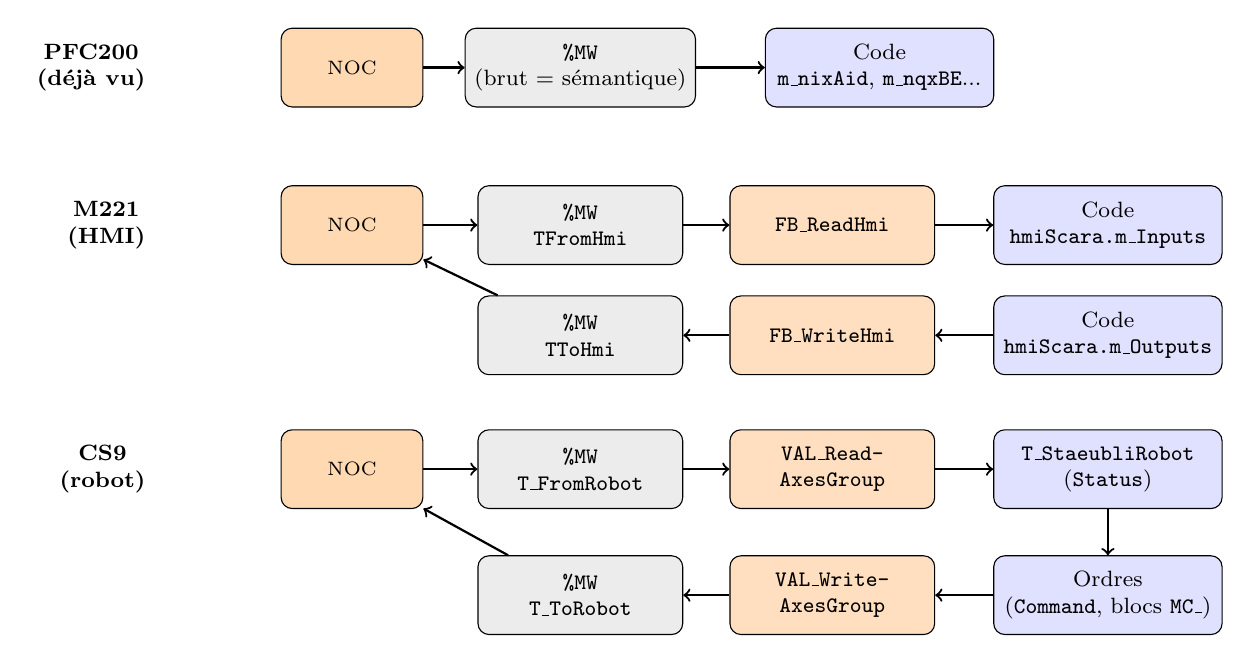
\begin{tikzpicture}[
        brut/.style = {draw, rounded corners, fill=gray!15, minimum width=2.6cm,
                        minimum height=1cm, align=center, font=\footnotesize},
        fb/.style = {draw, rounded corners, fill=orange!25, minimum width=2.6cm,
                        minimum height=1cm, align=center, font=\footnotesize},
        sem/.style = {draw, rounded corners, fill=blue!12, minimum width=2.9cm,
                        minimum height=1cm, align=center, font=\footnotesize},
        noc/.style = {draw, rounded corners, fill=orange!30, minimum width=1.8cm,
                        minimum height=1cm, align=center, font=\scriptsize},
        lien/.style = {thick, ->},
        rowlabel/.style = {font=\bfseries\footnotesize, anchor=east, align=center},
        ]

        % --- Ligne 1 : PFC200 (rappel, un seul niveau) ---
        \node[rowlabel] (lbl1) at (-6.3, 4) {PFC200\\(déjà vu)};
        \node[noc]  (noc1)  at (-3.8, 4) {NOC};
        \node[brut] (mw1)   at (-0.9,   4) {\texttt{\%MW}\\(brut = sémantique)};
        \node[sem]  (code1) at ( 2.9, 4) {Code\\\texttt{m\_nixAid}, \texttt{m\_nqxBE}...};
        \draw[lien] (noc1) -- (mw1);
        \draw[lien] (mw1) -- (code1);

        % --- Ligne 2 : M221 (HMI) ---
        \node[rowlabel] (lbl2) at (-6.3, 2) {M221\\(HMI)};
        \node[noc]  (noc2)  at (-3.8, 2) {NOC};
        \node[brut] (mw2)   at (-0.9, 2) {\texttt{\%MW}\\\texttt{TFromHmi}};
        \node[fb]   (fb2)   at ( 2.3, 2) {\texttt{FB\_ReadHmi}};
        \node[sem]  (code2) at ( 5.8, 2) {Code\\\texttt{hmiScara.m\_Inputs}};
        \draw[lien] (noc2) -- (mw2);
        \draw[lien] (mw2) -- (fb2);
        \draw[lien] (fb2) -- (code2);

        \node[sem]  (code2b) at ( 5.8, 0.6) {Code\\\texttt{hmiScara.m\_Outputs}};
        \node[fb]   (fb2b)   at ( 2.3, 0.6) {\texttt{FB\_WriteHmi}};
        \node[brut] (mw2b)   at (-0.9, 0.6) {\texttt{\%MW}\\\texttt{TToHmi}};
        \draw[lien] (code2b) -- (fb2b);
        \draw[lien] (fb2b) -- (mw2b);
        \draw[lien] (mw2b) -- (noc2);

        % --- Ligne 3 : CS9 (robot) ---
        \node[rowlabel] (lbl3) at (-6.3, -1.1) {CS9\\(robot)};
        \node[noc]  (noc3)  at (-3.8, -1.1) {NOC};
        \node[brut] (mw3)   at (-0.9, -1.1) {\texttt{\%MW}\\\texttt{T\_FromRobot}};
        \node[fb]   (fb3)   at ( 2.3, -1.1) {\texttt{VAL\_Read-}\\\texttt{AxesGroup}};
        \node[sem]  (code3) at ( 5.8, -1.1) {\texttt{T\_StaeubliRobot}\\(\texttt{Status})};
        \draw[lien] (noc3) -- (mw3);
        \draw[lien] (mw3) -- (fb3);
        \draw[lien] (fb3) -- (code3);

        \node[sem]  (ordres) at ( 5.8, -2.7) {Ordres\\(\texttt{Command}, blocs \texttt{MC\_})};
        \node[fb]   (fb3b)   at ( 2.3, -2.7) {\texttt{VAL\_Write-}\\\texttt{AxesGroup}};
        \node[brut] (mw3b)   at (-0.9, -2.7) {\texttt{\%MW}\\\texttt{T\_ToRobot}};
        \draw[lien] (code3) -- (ordres);
        \draw[lien] (ordres) -- (fb3b);
        \draw[lien] (fb3b) -- (mw3b);
        \draw[lien] (mw3b) -- (noc3);

    \end{tikzpicture}}
    \caption{Chaîne de conversion NOC $\to$ mémoire $\to$ code applicatif, selon l'équipement}
    \label{figChaineConversion}
\end{figure}

\begin{UPSTIinfor}{Ce que montre ce schéma}
Sur les trois équipements, l'alias mémoire sur la zone \texttt{\%MW} reste
le point d'entrée/sortie unique. Ce qui change, c'est ce qu'il faut faire
\emph{après} cet alias : rien de plus pour le PFC200, un passage par un
bloc fonctionnel de conversion pour le M221 et pour la baie CS9. Dans ce
dernier cas, le même objet sémantique (\texttt{T\_StaeubliRobot}) sert à
la fois à \textbf{lire} l'état du robot et à \textbf{lui donner des
ordres} : c'est pour cela qu'il est passé en \texttt{VAR\_IN\_OUT} aux
deux blocs \texttt{VAL\_Read/WriteAxesGroup}, et non simplement en entrée
ou en sortie.
\end{UPSTIinfor}

\begin{UPSTIactivite}[4][Suivre une information le long de la chaîne][][][TD]
\UPSTIquestion{L'opérateur appuie sur le bouton-poussoir « J3 : Up » du
pupitre. En s'appuyant sur la figure~\ref{figChaineConversion}, citer
dans l'ordre les objets et blocs traversés par cette information, depuis
le coupleur \texttt{NOC\_ETHIP\_ROBOT} jusqu'au champ
\texttt{hmiScara.m\_Inputs.m\_nixJ3Up} lu par le programme applicatif.}
\UPSTIquadrillage{3}

\begin{UPSTIcorrectionP}{Corrigé}
Coupleur \texttt{NOC\_ETHIP\_ROBOT} (connexion avec le M221) $\to$ zone
\texttt{\%MW} image des données reçues du M221 $\to$ alias
\texttt{fromHmiScara} (type \texttt{TFromHmi}, octets bruts) $\to$ bloc
\texttt{FB\_ReadHmi} (instance \texttt{InstReadHmi}, paramètre
\texttt{fromHmi}) $\to$ objet sémantique \texttt{hmiScara} (type
\texttt{THmi}), champ \texttt{hmiScara.m\_Inputs.m\_nixJ3Up}.
\end{UPSTIcorrectionP}

\UPSTIquestion{Faire de même pour la position cartésienne du robot
affichée sur l'écran du pupitre : depuis la baie CS9 jusqu'au M221. Quel
objet sémantique sert de « pont » entre la chaîne du robot et celle de
l'IHM ?}
\UPSTIquadrillage{4}

\begin{UPSTIcorrectionP}{Corrigé}
Baie CS9 (serveur \texttt{uniVALplc}) $\to$ coupleur
\texttt{NOC\_ETHIP\_ROBOT} $\to$ zone \texttt{\%MW}, alias
\texttt{fromRobotScara} (\texttt{T\_FromRobot}) $\to$
\texttt{VAL\_ReadAxesGroup} (paramètre \texttt{IN}) $\to$
\texttt{staeubliRobotScara.Status.CartesianPos} (\texttt{T\_StaeubliRobot})
$\to$ \texttt{FB\_WriteHmi} (paramètre \texttt{AxesGroup}), qui construit
$\to$ \texttt{toHmiScara} (\texttt{TToHmi}, sortie \texttt{toHmi}) $\to$
zone \texttt{\%MW} $\to$ coupleur \texttt{NOC\_ETHIP\_ROBOT} $\to$ M221
(écran du pupitre).

L'objet « pont » est \texttt{staeubliRobotScara} (type
\texttt{T\_StaeubliRobot}) : mis à jour par \texttt{VAL\_ReadAxesGroup}, il
est transmis sur le paramètre \texttt{AxesGroup} des blocs
\texttt{FB\_ReadHmi}/\texttt{FB\_WriteHmi}, d'où l'ordre d'appel imposé
(après \texttt{VAL\_ReadAxesGroup}).
\end{UPSTIcorrectionP}
\end{UPSTIactivite}

\pagebreak
\section{TD d'application : mode A6, mise en conditions initiales}
\label{secTdA6}

\begin{UPSTIinfor}{Objectif}
Mettre en œuvre le mode GEMMA \textbf{A6} du robot, en mobilisant la
chaîne de conversion présentée ci-dessus. Les trous proposés sont de
taille croissante : les premiers portent sur les blocs de
\textbf{conversion} déjà présentés en détail, les derniers vous demandent
de \textbf{choisir vous-même} le mouvement le plus adapté.
\end{UPSTIinfor}

\subsection{Rappel du comportement attendu (mode A6)}

Le robot doit rejoindre sa position de référence au-dessus du guichet,
sans jamais entraver la circulation des palettes sur le convoyeur :

\begin{enumerate}
    \item monter l'axe \textbf{J3} (vertical) jusqu'à $Z=150\;\text{mm}$,
    sans modifier la position courante des autres axes ;
    \item rejoindre ensuite la position cartésienne complète
    $(X=90,\ Y=-410,\ Z=150,\ RX=-180,\ RY=0,\ RZ=0)$.
\end{enumerate}

Si un arrêt est demandé par l'opérateur pendant ce mode, le robot doit
être immobilisé (sans perdre la puissance) puis reprendre sa course dès
que la demande d'arrêt n'est plus active. Ce bouton est accessible dans
l'objet \texttt{hmiScara} via
\texttt{hmiScara.m\_Inputs.m\_nixStopRequest} : comme rappelé en
section~\ref{secConversionHmi}, ce contact est à ouverture (\emph{NC}),
donc un arrêt est \textbf{demandé} lorsque ce booléen vaut
\texttt{FALSE}.

\subsection{Blocs utilisés dans ce TD}

Les blocs \texttt{MC\_} de contrôle et de commande de mouvement partagent
tous le même objet \texttt{AxesGroup} (\texttt{T\_StaeubliRobot}, déjà
lu/écrit par \texttt{VAL\_ReadAxesGroup}/\texttt{VAL\_WriteAxesGroup}) et
un squelette d'entrées/sorties commun :

\begin{center}
\begin{tabular}{|l|l|p{7.5cm}|}
\hline
\textbf{Paramètre} & \textbf{Sens / type} & \textbf{Rôle} \\
\hline
\texttt{Execute} & \texttt{VAR\_INPUT}, \texttt{BOOL} & Déclenche
l'exécution sur \textbf{front montant}. \\
\hline
\texttt{AxesGroup} & \texttt{VAR\_IN\_OUT}, \texttt{T\_StaeubliRobot} &
Objet du robot, commun à tous les blocs \texttt{MC\_}. \\
\hline
\texttt{Busy} / \texttt{Done} / \texttt{Error} & \texttt{VAR\_OUTPUT},
\texttt{BOOL} & En cours d'exécution / terminé avec succès / terminé en
erreur. \\
\hline
\end{tabular}
\end{center}

Les blocs de \textbf{mouvement} (\texttt{MC\_MoveLinearAbsolute},
\texttt{MC\_MoveDirectAbsolute}) ajoutent notamment, en \texttt{VAR\_INPUT} :
\texttt{Position} (\texttt{T\_CartesianPos}, la cible), \texttt{Velocity},
\texttt{Acceleration}, \texttt{Deceleration} (en~\% de la valeur
nominale), \texttt{CartesianVel}/\texttt{RotationalVel} (vitesses max. du
TCP) et \texttt{CoordSystem}/\texttt{ToolNumber} (repère et outil utilisés
-- \texttt{0} désigne respectivement le repère \texttt{world} et l'outil
\texttt{flange}).

\texttt{MC\_GroupPower} n'a qu'une entrée \texttt{Enable} (pas
\texttt{Execute}) et une seule sortie \texttt{Status} (état effectif de la
puissance) en plus d'\texttt{Error}/\texttt{ErrorID} -- il n'a pas de
notion de front, le bras reste sous/hors puissance tant que
\texttt{Enable} est à \texttt{TRUE}/\texttt{FALSE}.

\texttt{MC\_GroupInterrupt} et \texttt{MC\_GroupContinue} suivent le
squelette commun (\texttt{Execute}, \texttt{AxesGroup}, \texttt{Busy},
\texttt{Done}, \texttt{Error}) : le premier arrête le mouvement en cours
\emph{sans} vider la pile de commandes, le second relance l'exécution de
cette pile.

\UPSTIremarque[Objet \texttt{TCtrlStatusGroup}]{Par souci de lisibilité,
les sorties \texttt{Busy}/\texttt{Done}/\texttt{Error}/\texttt{ErrorID} de
ces blocs sont habituellement regroupées, lors de l'appel, dans un objet
de type \texttt{TCtrlStatusGroup} (champs \texttt{m\_xEnable},
\texttt{m\_xBusy}, \texttt{m\_xDone}, \texttt{m\_xError},
\texttt{m\_udiErrorID}, \texttt{m\_xTimeOut}) -- même logique que pour
\texttt{THmi} en section~\ref{secConversionHmi} : un seul objet nommé
plutôt que de nombreuses variables éparpillées.}

\subsection{Niveau 1 -- Compléter les blocs de conversion}

\begin{UPSTIactivite}[4][Appel de \texttt{VAL\_ReadAxesGroup} et \texttt{VAL\_WriteAxesGroup}][][][TD]
\UPSTIquestion{Compléter les paramètres manquants (repérés par
\texttt{(* A\_COMPLETER *)}) dans la section \texttt{ReadEthIpRobot} et
dans la section \texttt{WriteEthIpRobot} ci-dessous.}

\begin{lstlisting}
(* Section ReadEthIpRobot -- premiere section executee dans le cycle *)
InstReadAxesGroup(
    Enable     := (* A_COMPLETER *),
    AxesGroup  := (* A_COMPLETER *),
    IN         := fromRobotScara
);

(* ... section WriteEthIpRobot -- derniere section executee dans le cycle *)
InstWriteAxesGroup(
    Enable     := NOC_ETHIP_ROBOT_IN.HEALTH_BITS_IN[0].0,
    AxesGroup  := staeubliRobotScara,
    OUT        => (* A_COMPLETER *)
);
\end{lstlisting}
\vspace{2cm}
\end{UPSTIactivite}

\subsection{Niveau 2 -- Compléter la mise sous puissance}

\begin{UPSTIactivite}[4][Mise sous puissance du robot][][][TD]
\UPSTIquestion{Le robot doit rester sous puissance pendant toute la durée
du mode A6. Compléter l'appel au bloc \texttt{MC\_GroupPower}
ci-dessous : l'entrée \texttt{Enable} doit être activée en permanence
dans ce mode, et l'objet \texttt{AxesGroup} doit être celui de la cellule.}

\begin{lstlisting}
InstGroupPowerA6(
    Enable     := (* A_COMPLETER : toujours actif en mode A6 *),
    AxesGroup  := (* A_COMPLETER *)
);
\end{lstlisting}
\vspace{2cm}
\end{UPSTIactivite}

\subsection{Niveau 3 -- Choisir et écrire les mouvements}

À ce stade, vous disposez de tous les éléments pour écrire vous-même la
séquence de mouvement. Deux blocs \texttt{MC\_} vus en TP peuvent
convenir : \texttt{MC\_MoveLinearAbsolute} (mouvement linéaire) et
\texttt{MC\_MoveDirectAbsolute} (interpolation articulaire vers une
position cartésienne cible).

\begin{UPSTIactivite}[4][Étape 1 -- monter l'axe J3][][][TD]
\UPSTIquestion{L'énoncé demande de monter l'axe \textbf{J3} à
$Z=150\;\text{mm}$ \textbf{sans modifier la position courante des autres
axes}. Sur un robot Scara, l'axe J3 est l'axe vertical : une cible
cartésienne qui ne change que $Z$, en conservant $X$, $Y$, $RX$, $RY$,
$RZ$ courants, produit exactement ce déplacement.

\begin{enumerate}
    \item Entre \texttt{MC\_MoveLinearAbsolute} et
    \texttt{MC\_MoveDirectAbsolute}, quel bloc choisissez-vous pour cette
    étape ? Justifier à partir de la trajectoire que doit suivre l'outil
    (une translation verticale pure, sans contrainte angulaire
    particulière).
    \item Écrire, en complétant le squelette ci-dessous, l'instanciation
    et l'appel de ce bloc. La position cible utilisera les coordonnées
    \textbf{courantes} du robot pour $X$, $Y$, $RX$, $RY$, $RZ$ (déjà
    disponibles dans \texttt{staeubliRobotScara.Status.CartesianPos}), et
    $Z=150$.
\end{enumerate}}

\begin{lstlisting}
targetPosA6Etape1.X  := staeubliRobotScara.Status.CartesianPos.X;
targetPosA6Etape1.Y  := (* A_COMPLETER *);
targetPosA6Etape1.Z  := (* A_COMPLETER : valeur numerique de l'enonce *);
targetPosA6Etape1.RX := (* A_COMPLETER *);
targetPosA6Etape1.RY := (* A_COMPLETER *);
targetPosA6Etape1.RZ := (* A_COMPLETER *);

(* A_COMPLETER : instanciation et appel du bloc MC_ choisi,
   avec Execute, AxesGroup et la position cible ci-dessus *)
\end{lstlisting}
\vspace{3cm}
\end{UPSTIactivite}

\begin{UPSTIactivite}[4][Étape 2 -- rejoindre la position de référence][][][TD]
\UPSTIquestion{La position de référence
$(X=90,\ Y=-410,\ Z=150,\ RX=-180,\ RY=0,\ RZ=0)$ doit être rejointe par
une commande de mouvement \textbf{articulaire} (imposée par l'énoncé du
mode A6, contrairement à l'étape~1 où le choix était à justifier). Écrire
entièrement l'appel du bloc \texttt{MC\_} correspondant. Vous déclarerez
vous-même l'instance du bloc et la variable de position cible.}
\vspace{6cm}
\end{UPSTIactivite}

\begin{UPSTIactivite}[4][Gestion de l'arrêt demandé][][][TD]
\UPSTIquestion{Parmi les blocs \texttt{MC\_GroupInterrupt} et
\texttt{MC\_GroupContinue} vus en TP, lequel utiliser pour immobiliser le
robot sans perdre la puissance lorsqu'un arrêt est demandé, et lequel
pour reprendre la course lorsqu'il ne l'est plus ? Rédiger les deux
conditions d'appel (sur l'entrée \texttt{Execute} de chaque bloc, sans
écrire l'instanciation complète), en utilisant
\texttt{hmiScara.m\_Inputs.m\_nixStopRequest}.}
\vspace{4cm}
\end{UPSTIactivite}



\end{document}
